\documentclass[10pt,a4paper,oneside,titlepage]{report}
\usepackage[utf8]{inputenc}
\usepackage[english,russian]{babel}
\usepackage{amsmath}
\usepackage{amsthm}
\usepackage{amssymb}
\usepackage{cmll}
\usepackage{enumerate}
\usepackage{stmaryrd}
\usepackage[left=2cm,right=2cm,top=2cm,bottom=2cm,bindingoffset=0cm]{geometry}
\usepackage{url}
\usepackage{listingsutf8}
\usepackage{graphicx}
\graphicspath{{pictures/}}
\DeclareGraphicsExtensions{.pdf,.png,.jpg}

\lstset{%
	numbers = left
}

\title{Конспект по курсу Сети \thanks{Читаемый  в 2019-2020 годах}}
\author{Александра Лисицына \thanks{Студентка группы М3435}}

\theoremstyle{defenition}
\newtheorem*{defenition}{Определение}

\begin{document}
	
\maketitle

\tableofcontents

\clearpage	

\chapter{Введение}

\section{Модель OSI}

\begin{figure}[h!]
	\centering
	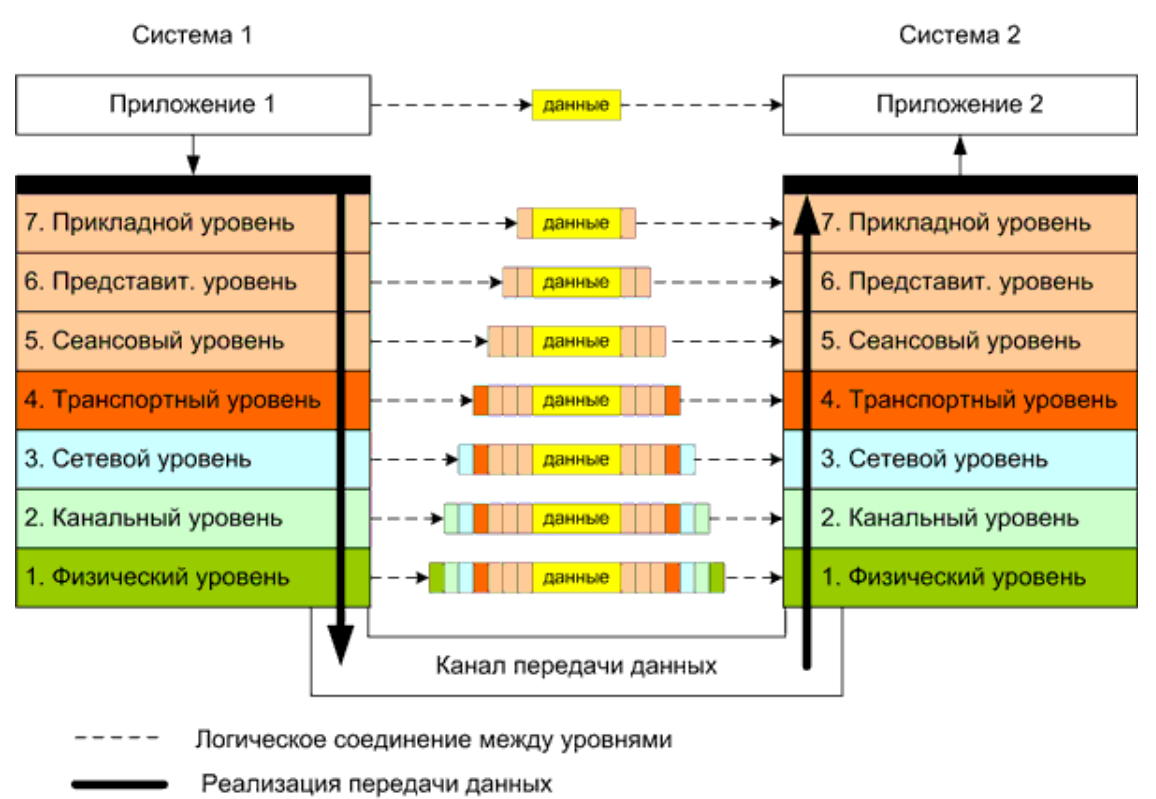
\includegraphics[width=0.4\linewidth]{pictures/ModelOSI}
	\caption[Модель OSI]{}
	\label{fig:modelosi}
\end{figure}


\section{Физический и канальный уровни корпоративных сетей}

\subsubsection{Стркутурированные кабельные системы} % (fold)

\section{Соединение IP сетей}

\subsection{Виды маршрутизации}

Маршрутизацию можно классифицировать двумя способами:
\begin{itemize}
	\item Статическая и динамическая
	\item Внешняя и внутренняя
\end{itemize}

Внешняя необходима для маршрутизации между автономными системами (EGP, BGP).

Внутрення --- внутри одной системы (RIP, OSPF).

OSPF -- открытие кратчайшего пути первым. Информации включения/отключения сетей пересылается сразу, по мере появления. По этой информации строится нагруженный граф сети (веса назначаются по таблице в зависимости от скорости линии связи). Маршрут считается по алгоритму Дириха. Быстрее получаем маршрутную информацию, понимаем скорости и быстро перестраиваем при ищменении конфигурации. Но его гораздо сложнее настраивать. 

Сеть в маршрутизации описывается в виде табоицы маршрутизации. 

В TCP/IP мы занимаемся каждым отдельным пакетом. В этом есть минус, так как обычно все пакеты дают один и тот же пакет.

Таблицы маршрутизации строит либо админ, либо протокол маршрутизации. 

\subsection{NAT (Network Address Translation)}

Основная причина появления --- постоянная нехватка IP адресов.

Не всем хостам нужен IP адрес, а использовать маршуртизацию нельзя.

Цель: обеспечить связь хостов из немаршуртизуемой сети во внешнюю IP сеть.

Виды:
\begin{itemize}
	\item Публикация адреса
	\item Клиентский NAT
	\item Публикация порта
\end{itemize}

\subsubsection{Публикация адреса}

Когда: Вы - провайдер домашнего интернета. И один из пользователей вашей сети захотел себе NAS (Network Attached Storage --- компьютер с диском, к которому мы ходим из разных мест по разным протоколам), ему нужен реальный IP адрес. Вариант с разделением всей сети масками очень сложен и плох. Поэтому мы делаем подстановку: маршуртизатор провайдера, когда получает пакет на реальный адрес, то меняет его на локальный и посылает по сети, обратно наоборот. Но эта схема работает только, если используется один алрес, для большего количества не работает.

%картинка

\subsubsection{Клиентский NAT}

%картинка


Плюсы: любое количество хостов можем выпустить наружу в интернет через один IP адрес.

\subsubsection{Публикация порта}

Теперь можно из интернета попасть на устройство. Нам нужен лишь один IP адрес. И обратившись на опубликованный сокет мы попадем на нужное кстройство. 

\end{document}
